\chapter{CNN classifier using transfer learning}\label{chapter5}
In order to choose a CNN model, we evaluated several contemporary architectures, as ResNeXt \cite{xie2017aggregated} or ConvNeXt \cite{liu2022convnet} and finally opted for an EfficientnetV2 architecture \cite{tan2021efficientnetv2}, a general purpose architecture proposed by Google researchers that showed excellent performance.

We present the design ideas behind the EfficientNet architecture and its adaptation to our current problem. We also evaluate the results of the model and some additional properties, like calibration.

\section{The EfficientNet architecture} \label{sec:efficientnet}
EfficientNet \cite{efficientNet, googleEfficient} is a family of models that emerged to improve the efficiency and accuracy of existing models by scaling an established model. It is common to scale convolutional neural networks once more resources are available, in order to improve performance. The conventional way to scale these models is to arbitrarily increase the different dimensions of the network, either the depth or the width or the resolution.

Unlike conventional methods, EfficientNet uses a novel way of scaling the model by uniformly resizing each dimension based on a fixed set of scaling coefficients. This strategy is very successful as EfficientNet significantly outperformed the state-of-art models.

The key of this model is to scale all the dimensions of the neural network (\Cref{fig:scaling}). In order to achieve this, an exhaustive search of the hyperparameters of the network is carried out to find the relationship between different scaling orders of each dimension in the base model under a set of restrictions. Once this search is performed, the scaling coefficient for each dimension is determined.

 \begin{figure}[tb]
    \centering
    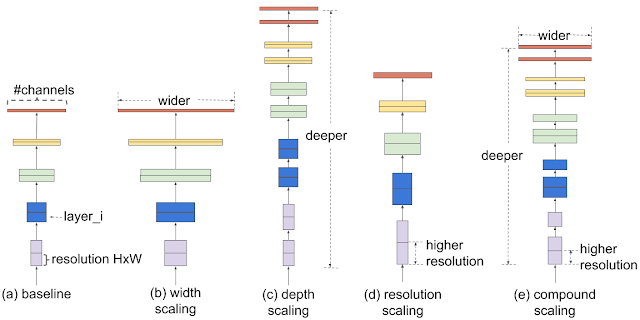
\includegraphics[width=\textwidth]{figures/chapter5/efficient/compoundScaling.png}
    \caption{Difference between traditional techniques for scaling CNNs (b), (c), (d) and the scaling method used by EfficientNet (e) \cite{efficientNet}.}
    \label{fig:scaling}
\end{figure}
The choice of the base model (a) is crucial. EfficientNet uses a technique for automating the design of artificial neural networks called Neural Architecture Search (NAS) \cite{white2023neural}, consistent in searching the model that maximizes a performance estimation over a predefined family of models. The result of this search is EfficientNet-B0, whose architecture is presented in \Cref{fig:baseline}. The rest of the models of the family are created by scaling the baseline using the previously found hyperparameters: the original family consisted of 7 additional models (from B1 to B7) ranging from the 5.3 million parameters of the backbone to 66 millions parameters for B7.

\begin{figure}[tb]
    \centering
    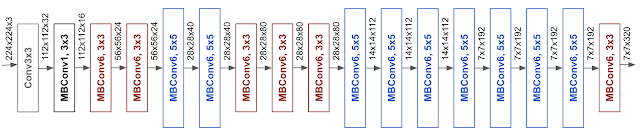
\includegraphics[width=\textwidth]{figures/chapter5/efficient/EfficientNetv0.png}
    \caption{Baseline Architecture}
    \label{fig:baseline}
\end{figure}

Presented in 2021, EfficientNetV2 proposes an improvement over the EfficientNet family, achieving higher parameter efficiency and higher training speed than other previous models and comparing favorably against much bigger vision transformer models such as ViT-L (\Cref{fig:comparison}). 
\begin{figure}[tbp]
    \centering
    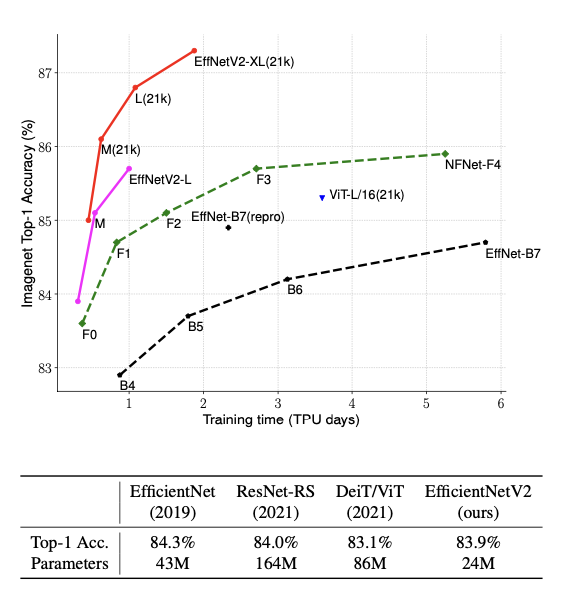
\includegraphics[width=0.6\textwidth]{figures/chapter5/efficient/graficaV2.png}
    \caption{Comparison with other models: EfficientNetV2 obtains better accuracy with a fraction of parameters and training time \cite{tan2021efficientnetv2}.}
    \label{fig:comparison}
\end{figure}

The creators of EfficientNetV2 maintained the original objective of EfficientNet: maximizing the parameter efficiency, in order to obtain state-of-the-art results with relatively small models. The v2 version pays especial attention to the problem of training, as the EfficientNet models required careful hyperparameter tuning and were not especially fast to train. EfficientNetV2 is up to 11 times faster training speed and 6.8 times more parameter efficiency in ImageNet, CIFAR, Cars and flowers datasets than the state of the art models \cite{tan2021efficientnetv2}, a speed-up that becomes more notable when using large resolution images.

The models of the v2 family are therefore excellent candidates for situations with limited computing power. The team designed the architecture around the main bottlenecks of EfficientNet. They found the following problems \cite{tan2021efficientnetv2}:

\begin{enumerate}
    \item Training using very large images is slow: EfficientNet's utilization of large image size results in significant memory usage. To alleviate the problem they propose to use \textit{progressive learning}, which involves progressively increasing the image size provided to the model. This approach exploits the fact that the use of global pooling makes the model agnostic about the input size.
    \item Depthwise convolutions show slower performance in the initial layers, but they are effective in later stages: these type of convolutions have fewer parameters and require fewer floating point operations per second compared to regular convolutions, but they often fail to fully leverage the capabilities of modern accelerators. The researchers proposed to alternate the use of different convolutional blocks (as Fused-MBconv and MBConv) and perform Neural Architecture Search to find the best combination to maintain the efficiency in parameters and make training faster.
    \item Scaling up each stage equally is suboptimal: EfficientNet scales all stages uniformly using a simple rule, but the stages don't contribute equally to the training speed or parameter efficiency.  However, EfficientNetsV2 use a non-uniform scaling strategy to progressively add more layers to the later stages. 
\end{enumerate}

The result of these improvements was a complete family of models comprising both minimal models (like EfficientNetV2-B0 with just 7.4 million of parameters) and very large models (like EfficientNetV2-XL, which has 208 million parameters).

\section{Model Architecture}\label{archModel}
The usual architecture for a vision model for classification is composed of a \textit{backbone} and a \textit{classifier}. The \textit{backbone} works as a \textit{feature extractor} that will encode the input into a feature representation. In the case of a convolutional neural network, the backbone is usually composed of a convolutional block and a \textit{global pool layer}, that will determine how the hidden channels of the representation are merged.

The \textit{classifier} is often a conventional neural network and can be substituted for other components to address other problems, usually maintaining the original backbone.

We will follow a similar architecture: the backbone of our model (\Cref{fig:architecture}) is an EfficientNetV2-B3 model, a medium-sized (14M parameters) architecture that presents a good compromise between accuracy and complexity. We used the implementation from the open source library timm \cite{timm} (Pytorch Image Models). 

Furthermore, we opted for a working resolution of 512 × 512, offering a good compromise between performance and efficiency. 

\begin{figure}[ht]
    \centering
    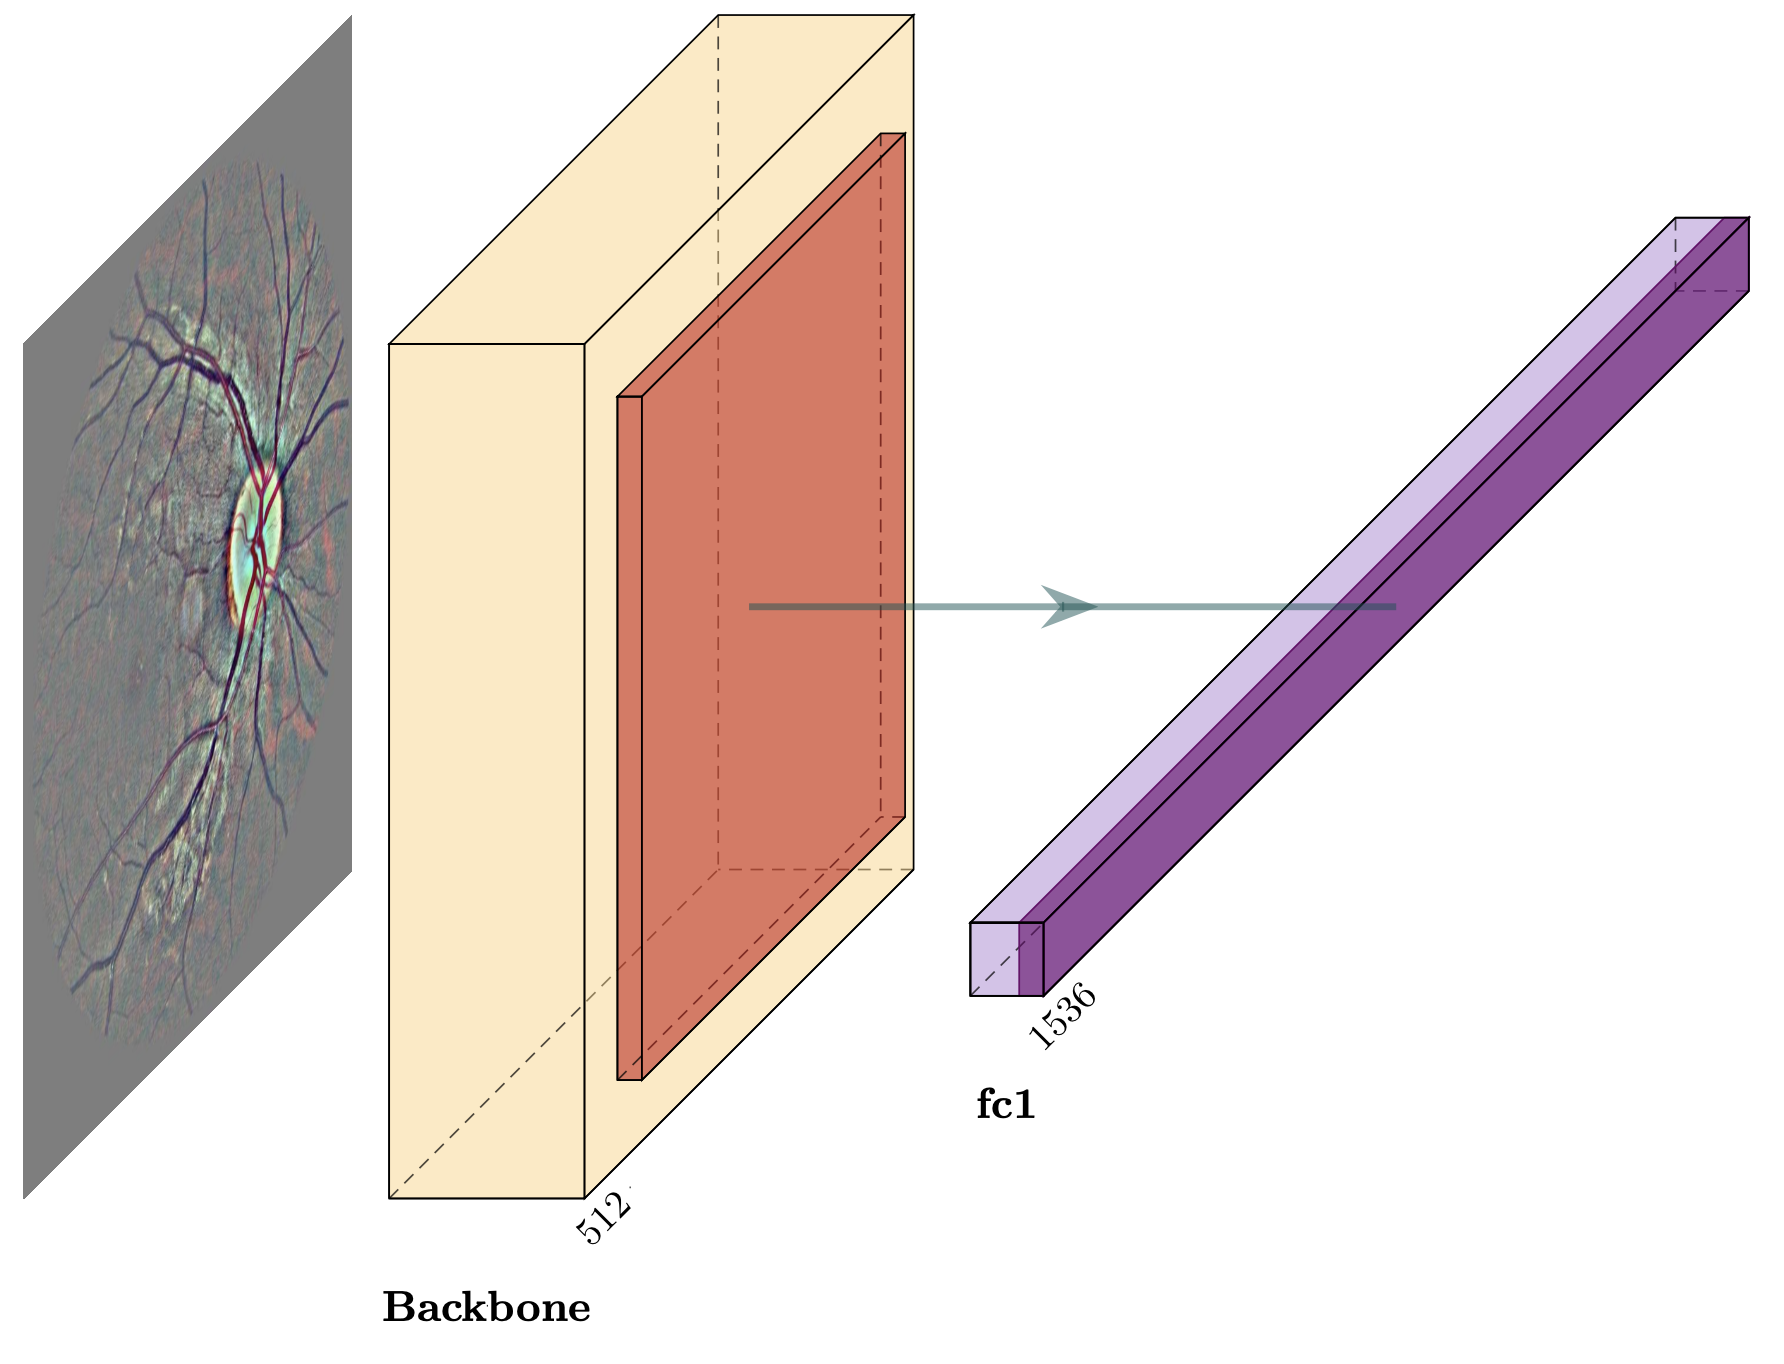
\includegraphics[scale=0.3]{figures/chapter5/models/model.png}
    \caption{Architecture of the model. The features extracted by the CNN are pooled using global average pooling before being flattened and fed to the classifier.}
    \label{fig:architecture}
\end{figure}

The backbone is fed each image and its output is pooled using \textit{global average pooling}, which reduces each channel of the output to a single scalar, by averaging all the components of the channel. We use as classifier a simple linear network which outputs the \textit{logits}, the unnormalized probabilities for each class.

\subsection{Transfer learning}
Since we were restricted to models that could be trained with limited computational resources, we opted to use a CNN and to apply transfer learning: using a model trained for one task (in the case of CNN, usually object detection in a general purpose dataset as ImageNet) and retrain it for a new task over the specific dataset (\textit{fine-tuning}).

Transfer learning has been proved to be a reliable way to save computational power even in the case that the original and the new datasets are quite different, apparently because features originally learned can be reused \cite{haslum2022makes}.

We use a backbone pretrained on ImageNet21K, a database with 21,000 general purpose images for image classification problems. In order to not destroy the original weights, we \textit{fine-tune} the model to the new database using a low learning rate. We opted for training the whole model (without freezing any layer), since the ImageNet database is quite different to the EyePACS one.

In our experiments, the pretrained model obtained an accuracy of 83.5\% after just one iteration, compared to just 52.6\% for the non-pretrained one, which suggests transfer learning is highly successful at reducing training time and easing convergence with almost none overhead.

\subsection{Training the model}
The model was trained using Adamax optimizer \cite{kingma2017adam} and unweighted Cross Entropy as the loss function. \Cref{table:adamax} shows the hyperparameters of the optimizer used for training, so the results can be reproduced.

We tried other strategies as alternative optimizers (Adam, SGD) as well as approaching the problem as a regression, but they offered poorer results. We did not find reliable strategies to improve the performance over under-represented classes. Both oversampling (showing the model more images from under-represented classes each epoch) and under-sampling (reducing the number of over-represented classes in the dataset) severely deteriorated performance both general and over under-represented classes. 

Weighting under-represented classes (so the loss for instances of underrepresented classes is weighted more than for instances of over-represented classes) also weakened the model performance.

\begin{figure}[tb]
     \begin{subfigure}[b]{0.65\textwidth}
        \centering
        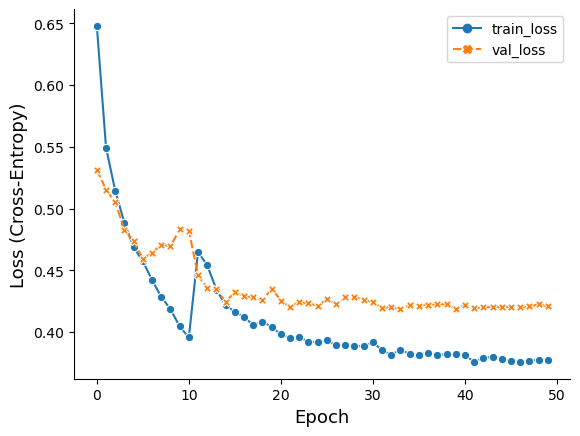
\includegraphics[width=\textwidth]{figures/chapter5/metrics/loss.png}
        \caption{Loss evolution during training.}
        \label{fig:training}
    \end{subfigure}
    \hfill
    \begin{subfigure}[b]{0.34\textwidth}
        \centering

        \resizebox{\columnwidth}{!}{
        \small
        \begin{tabular}{|cc|}
        \hline
        \multicolumn{2}{|c|}{Hyperparameters: Adamax} \\ \hline \hline
        Lr & 1e-2 \\ \hline
        $(\beta_1, \beta_2)$  & (0.9, 0.999)  \\  \hline
        $\epsilon$ & 1e-7 \\  \hline
        Weight decay & 1e-2 \\ \hline
        \end{tabular}
        }
        \caption{Hyperparameters used for training.}
        \label{table:adamax}
    \end{subfigure}
\end{figure}

We trained for 50 epochs in an Nvidia GTX 1070 GPU (approximately 9 hours). The results of training are shown in \Cref{fig:training}. We observed very fast convergence during the first epoch followed by \textit{overfitting}, that we addressed adding regularization in the form of weight decay and late dropout \cite{liu2023dropout} and reducing the learning rate, achieving model convergence. The evolution of the main indicators (accuracy, macro F1 and Cohen's Kappa coefficient) led us to think the model has a good performance in all classes. 

As it is common in the field, we used Cohen's kappa coefficient as the main measure of performance. This statistic estimates the accuracy of a rating by comparing it with the expected accuracy of a random rater \cite{cohen1960kappa}. 

\begin{figure}[tb]
     \centering
     \begin{subfigure}[b]{0.32\textwidth}
         \centering
         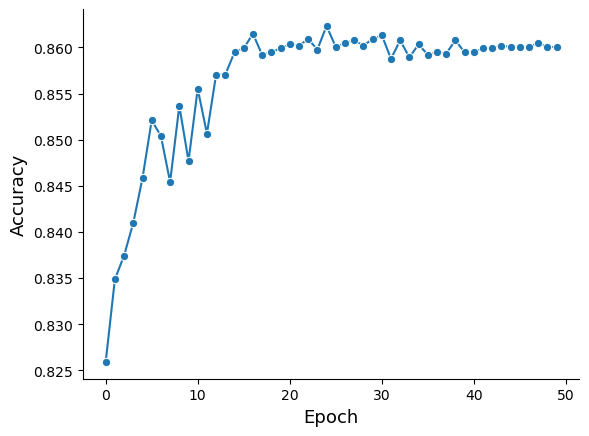
\includegraphics[width=\textwidth]{figures/chapter5/metrics/accuracy.png}
         \caption{Accuracy}
         \label{fig:accuracy}
     \end{subfigure}
     \hfill
     \begin{subfigure}[b]{0.32\textwidth}
         \centering
         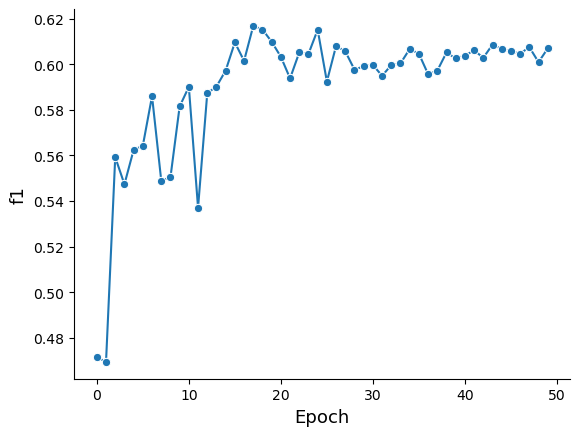
\includegraphics[width=\textwidth]{figures/chapter5/metrics/f1.png}
         \caption{F1 score}
         \label{fig:f1}
     \end{subfigure}
     \hfill
     \begin{subfigure}[b]{0.32\textwidth}
         \centering
         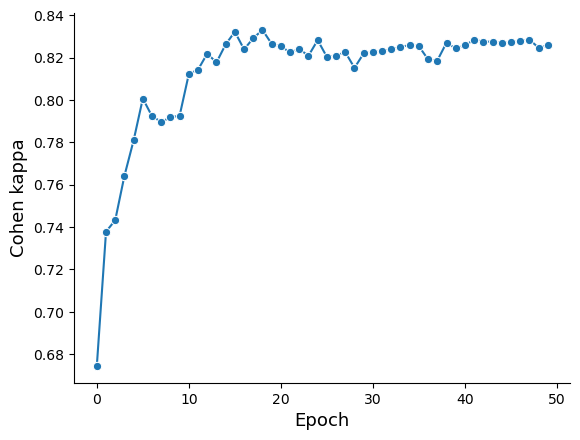
\includegraphics[width=\textwidth]{figures/chapter5/metrics/kappa.png}
         \caption{Cohen's $\kappa$}
         \label{fig:kappa}
     \end{subfigure}
        \caption{Performance of the model during training, measured by three metrics: accuracy, macro F1 score and squared Cohen kappa}
        \label{fig:metrics}
\end{figure}

\subsection{Calibrating the model}
In order to carry further analysis, it is convenient to be able to interpret the predictions of the model in terms of probabilities for each class.

It has been observed that most deep learning models tend to be overconfident and directly interpreting the results of the model as probabilities (by applying \textit{softmax} to the logits) will not reflect the true likelihood of the event \cite{guo2017calibration}.

In a well calibrated model, the probability associated with the predicted class label reflects its ground truth correctness likelihood.

To calibrate the model we use \textit{temperature scaling} \cite{guo2017calibration}, a method which estimates a constant \( T \) to scale the logits output by the model to minimize negative log likelihood over the validation set. After regularization, the probability of the classes is given by \( p = \softmax(y / T) \) where \( y \) are the logits of the model. In particular, temperature scaling does not affect the predictions made by the model as it does not alter the ratio between logits for different classes.

We used the implementation provided by the team responsible for the popularization of temperature scaling \cite{guo2017calibration}, which employs a neural network to estimate a value of \( T = 1.15 \).

\begin{figure}[tbp]
    \centering
    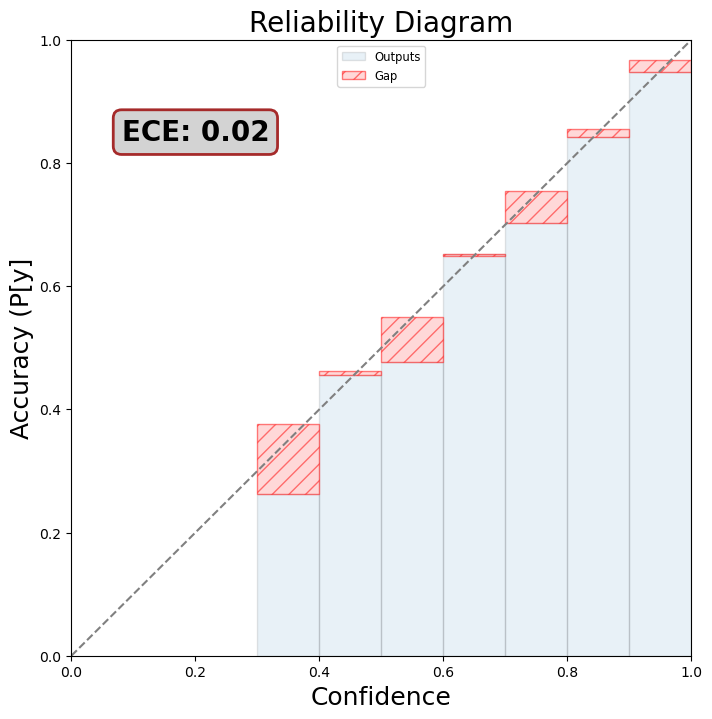
\includegraphics[scale = 0.45]{figures/chapter5/calibration/post_calibration.png}
    \caption{Reliability diagram after calibration. }
    \label{fig:reliability}
\end{figure}

The reliability diagram after normalization (\Cref{fig:reliability}) shows that the final model is relatively well calibrated and is quite precise for high levels of accuracy, although the model tends to be too unconfident about cases with low accuracy. 

The estimated calibration error (the expected value of the gap between confidence and accuracy) is just 0.02, which confirms the model is indeed well-calibrated.

We can use the calibrated probabilities to identify images that are particularly challenging to grade for the model (\Cref{fig:unconfident}). While some of these images are too noisy to be useful (\Cref{fig:unconfident0}), others pose a real challenge because of unusual framing or coloring, like \Cref{fig:unconfident3}. 

There are multiple use cases for images like these: for example, to test the performance of preprocessing methods over images with unusual characteristics or to implement educational tools for ophthalmology students. 

\begin{figure}[tb]
     \centering
     \begin{subfigure}[b]{0.32\textwidth}
         \centering
         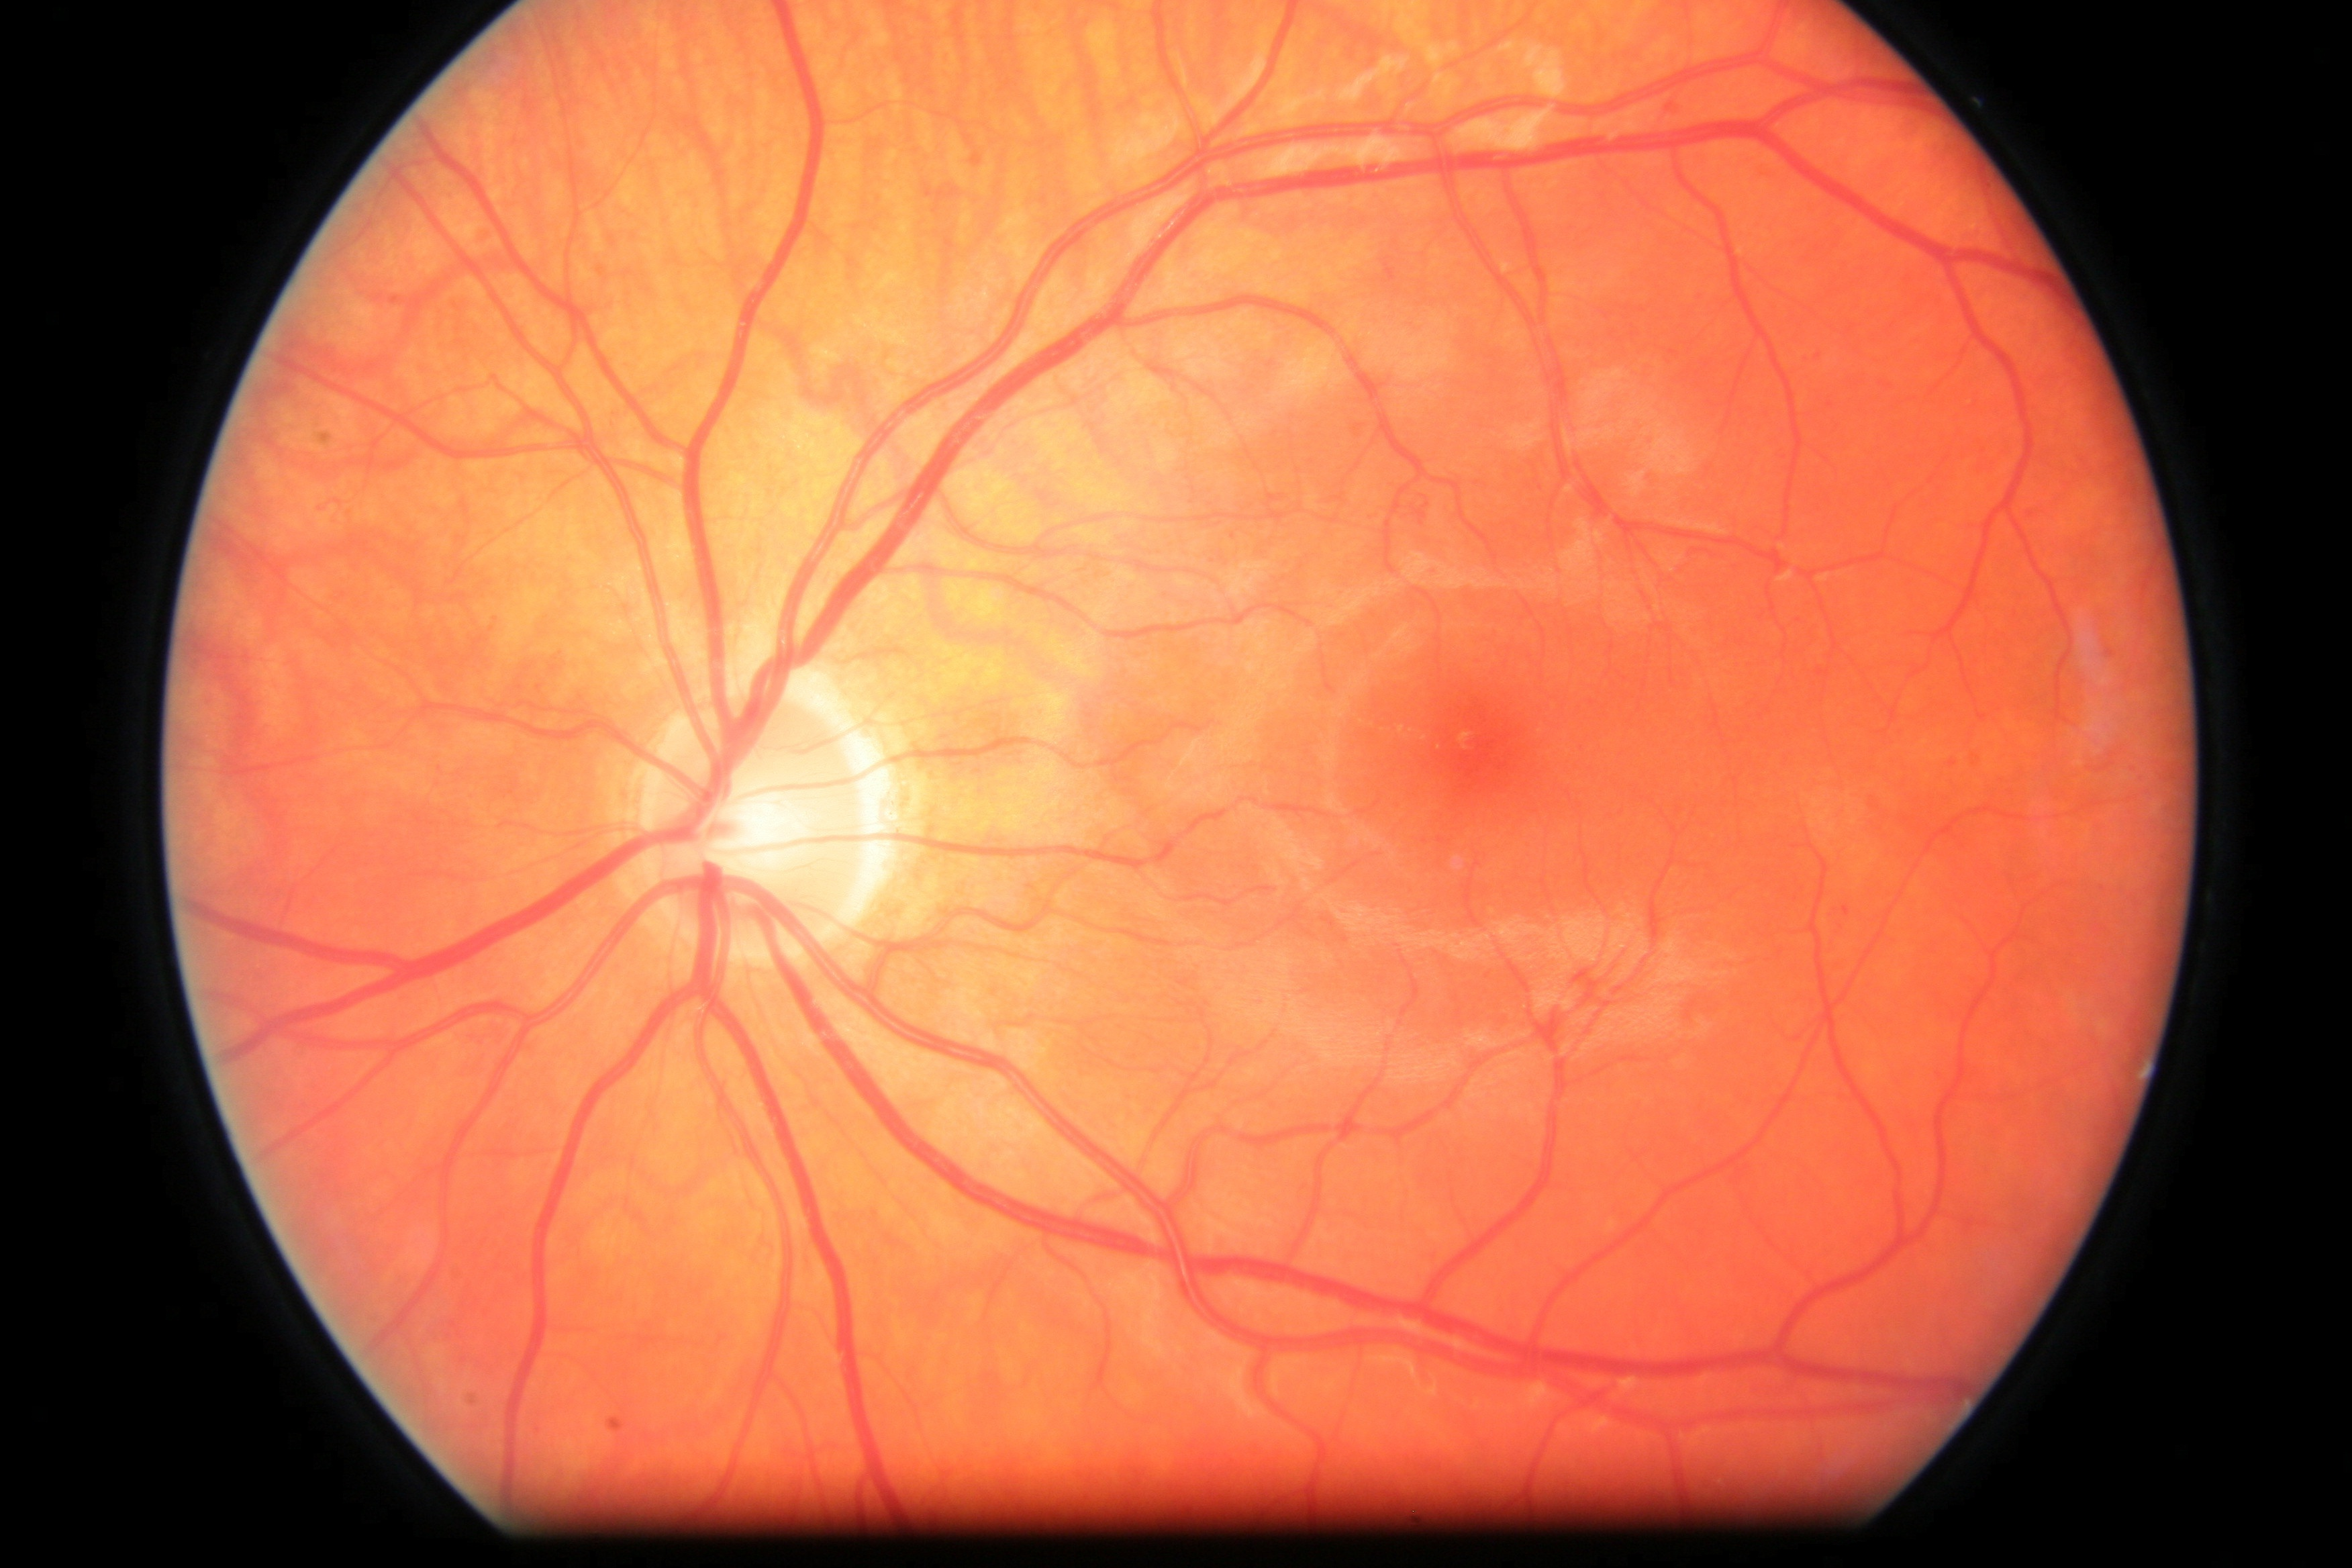
\includegraphics[height=\textwidth,width=\textwidth]{figures/chapter5/unconfident/10345_right.jpeg}
         \caption{Pred.: 1. Target: 2}
         \label{fig:unconfident0}
     \end{subfigure}
     \hfill
     \begin{subfigure}[b]{0.32\textwidth}
         \centering
         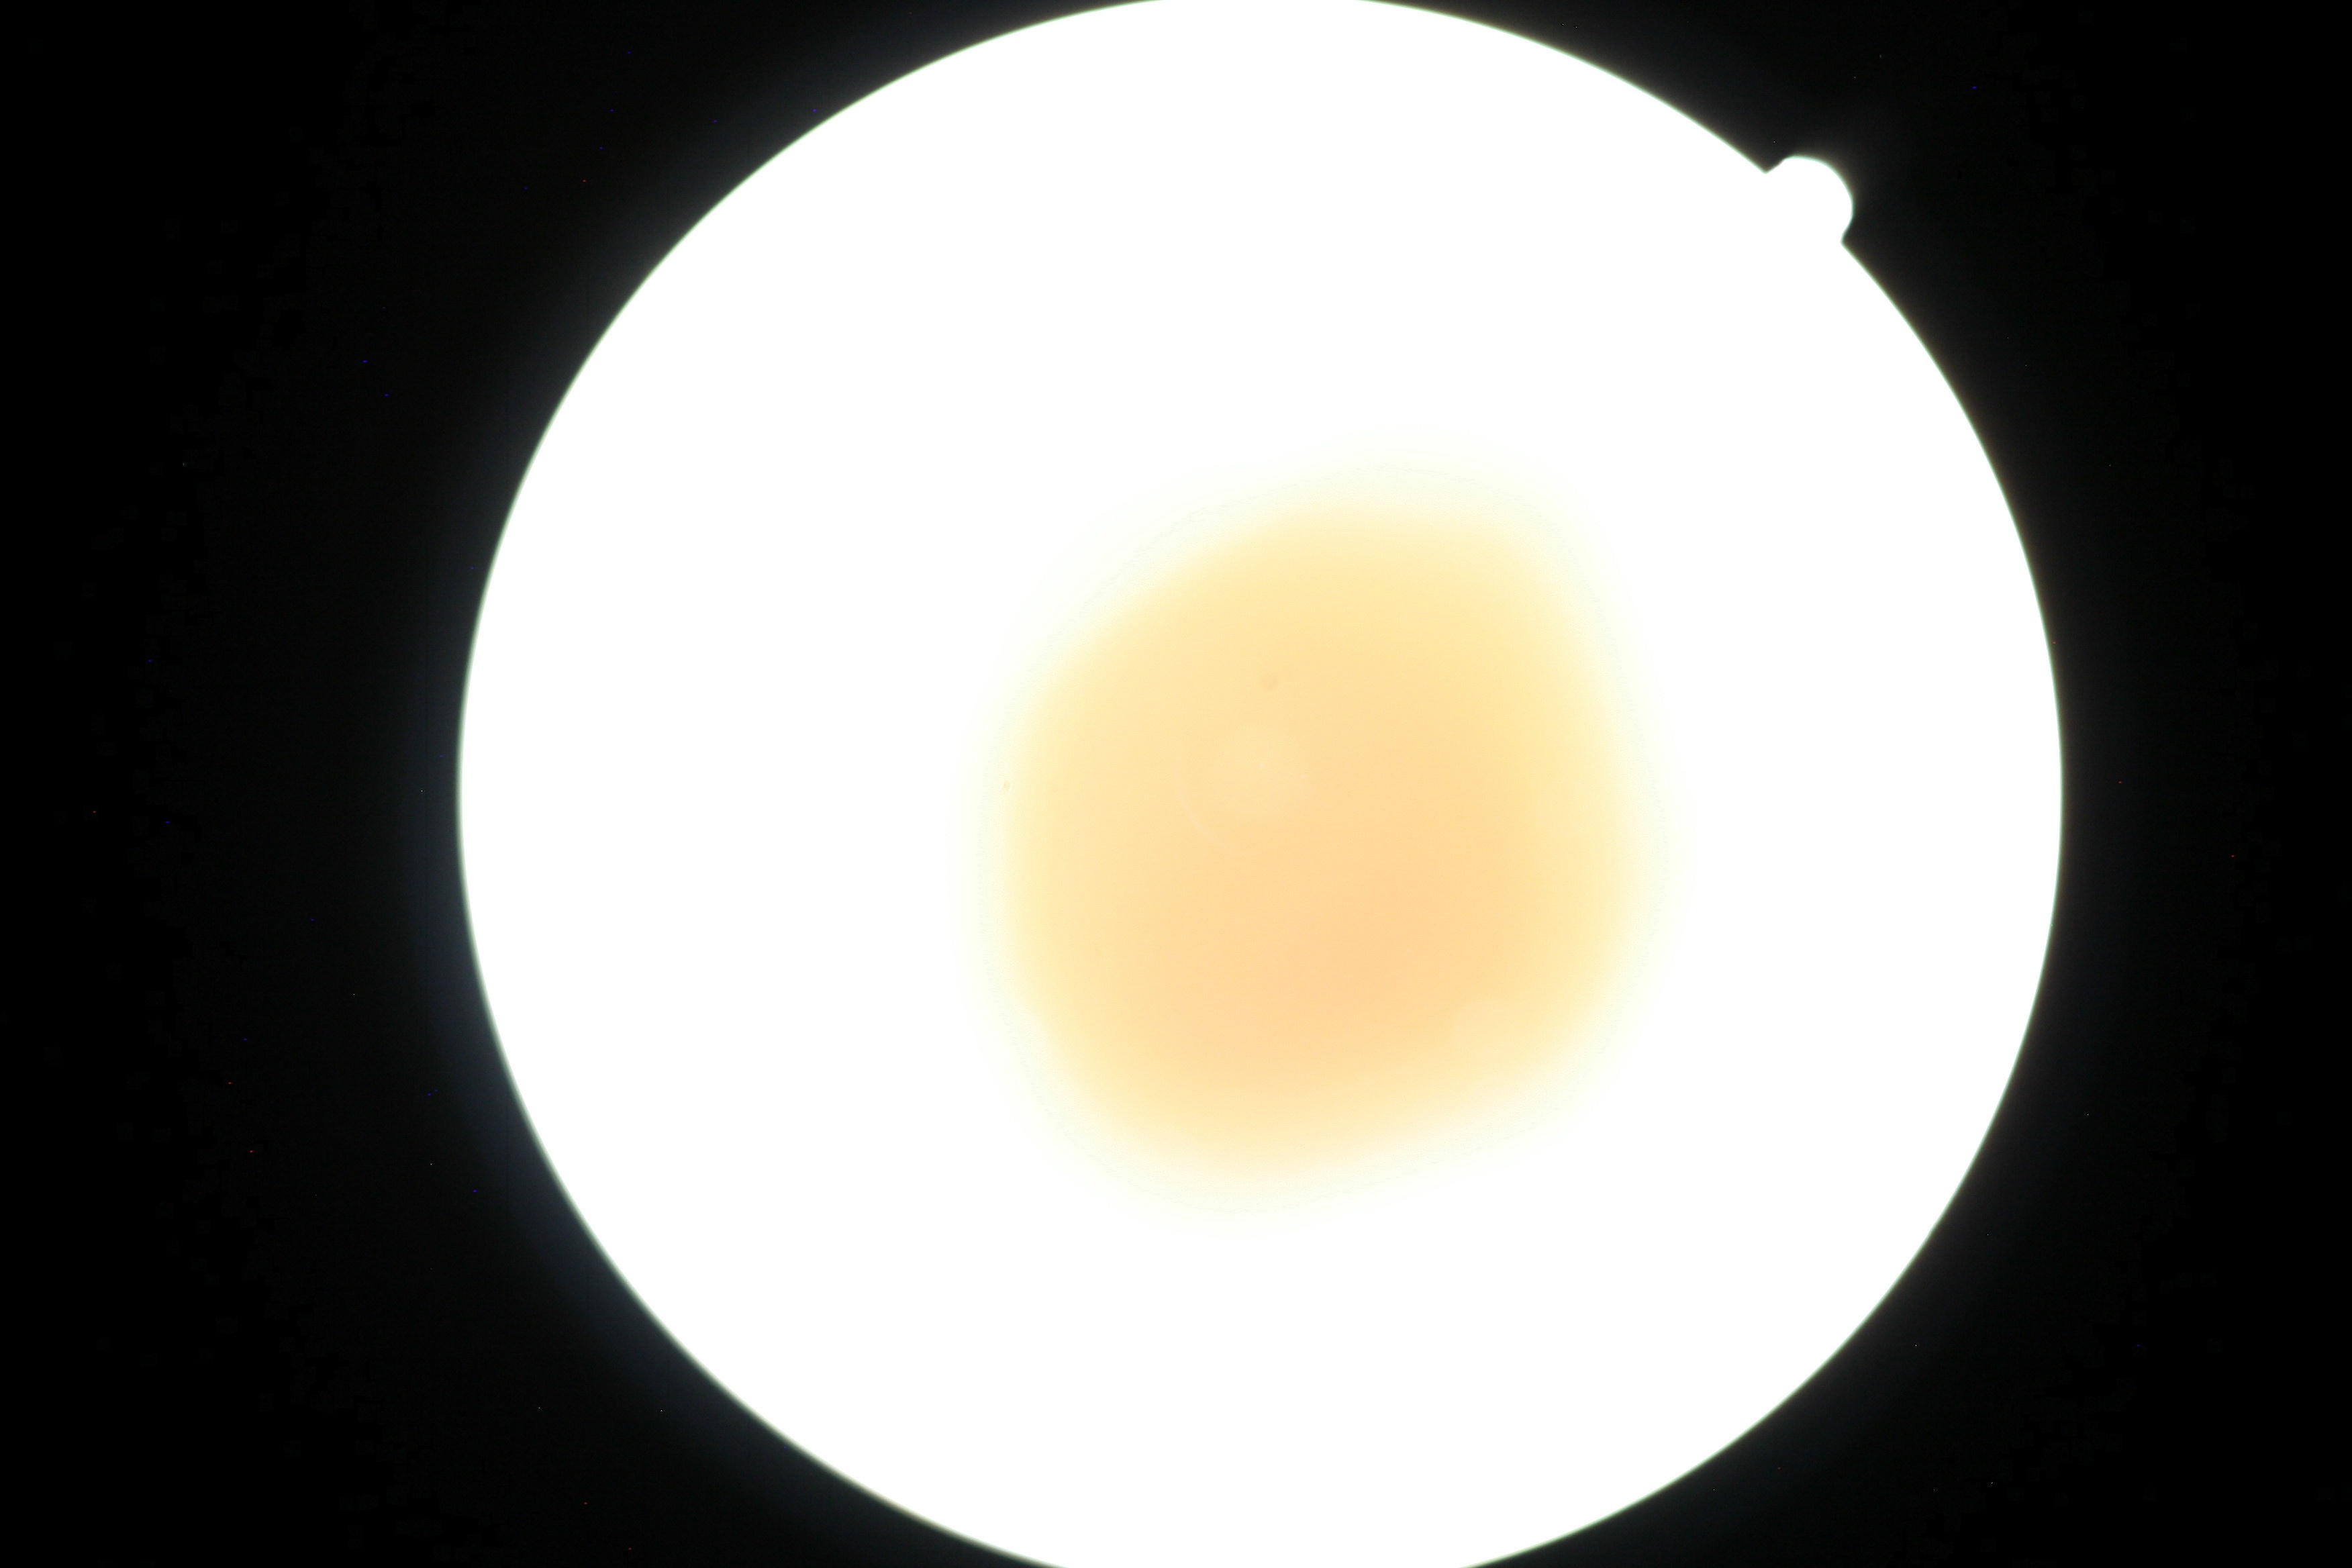
\includegraphics[height=\textwidth,width=\textwidth]{figures/chapter5/unconfident/3042_left.jpeg}
         \caption{Pred.: 0. Target: 2.}
     \end{subfigure}
     \hfill
    \begin{subfigure}[b]{0.32\textwidth}
         \centering
         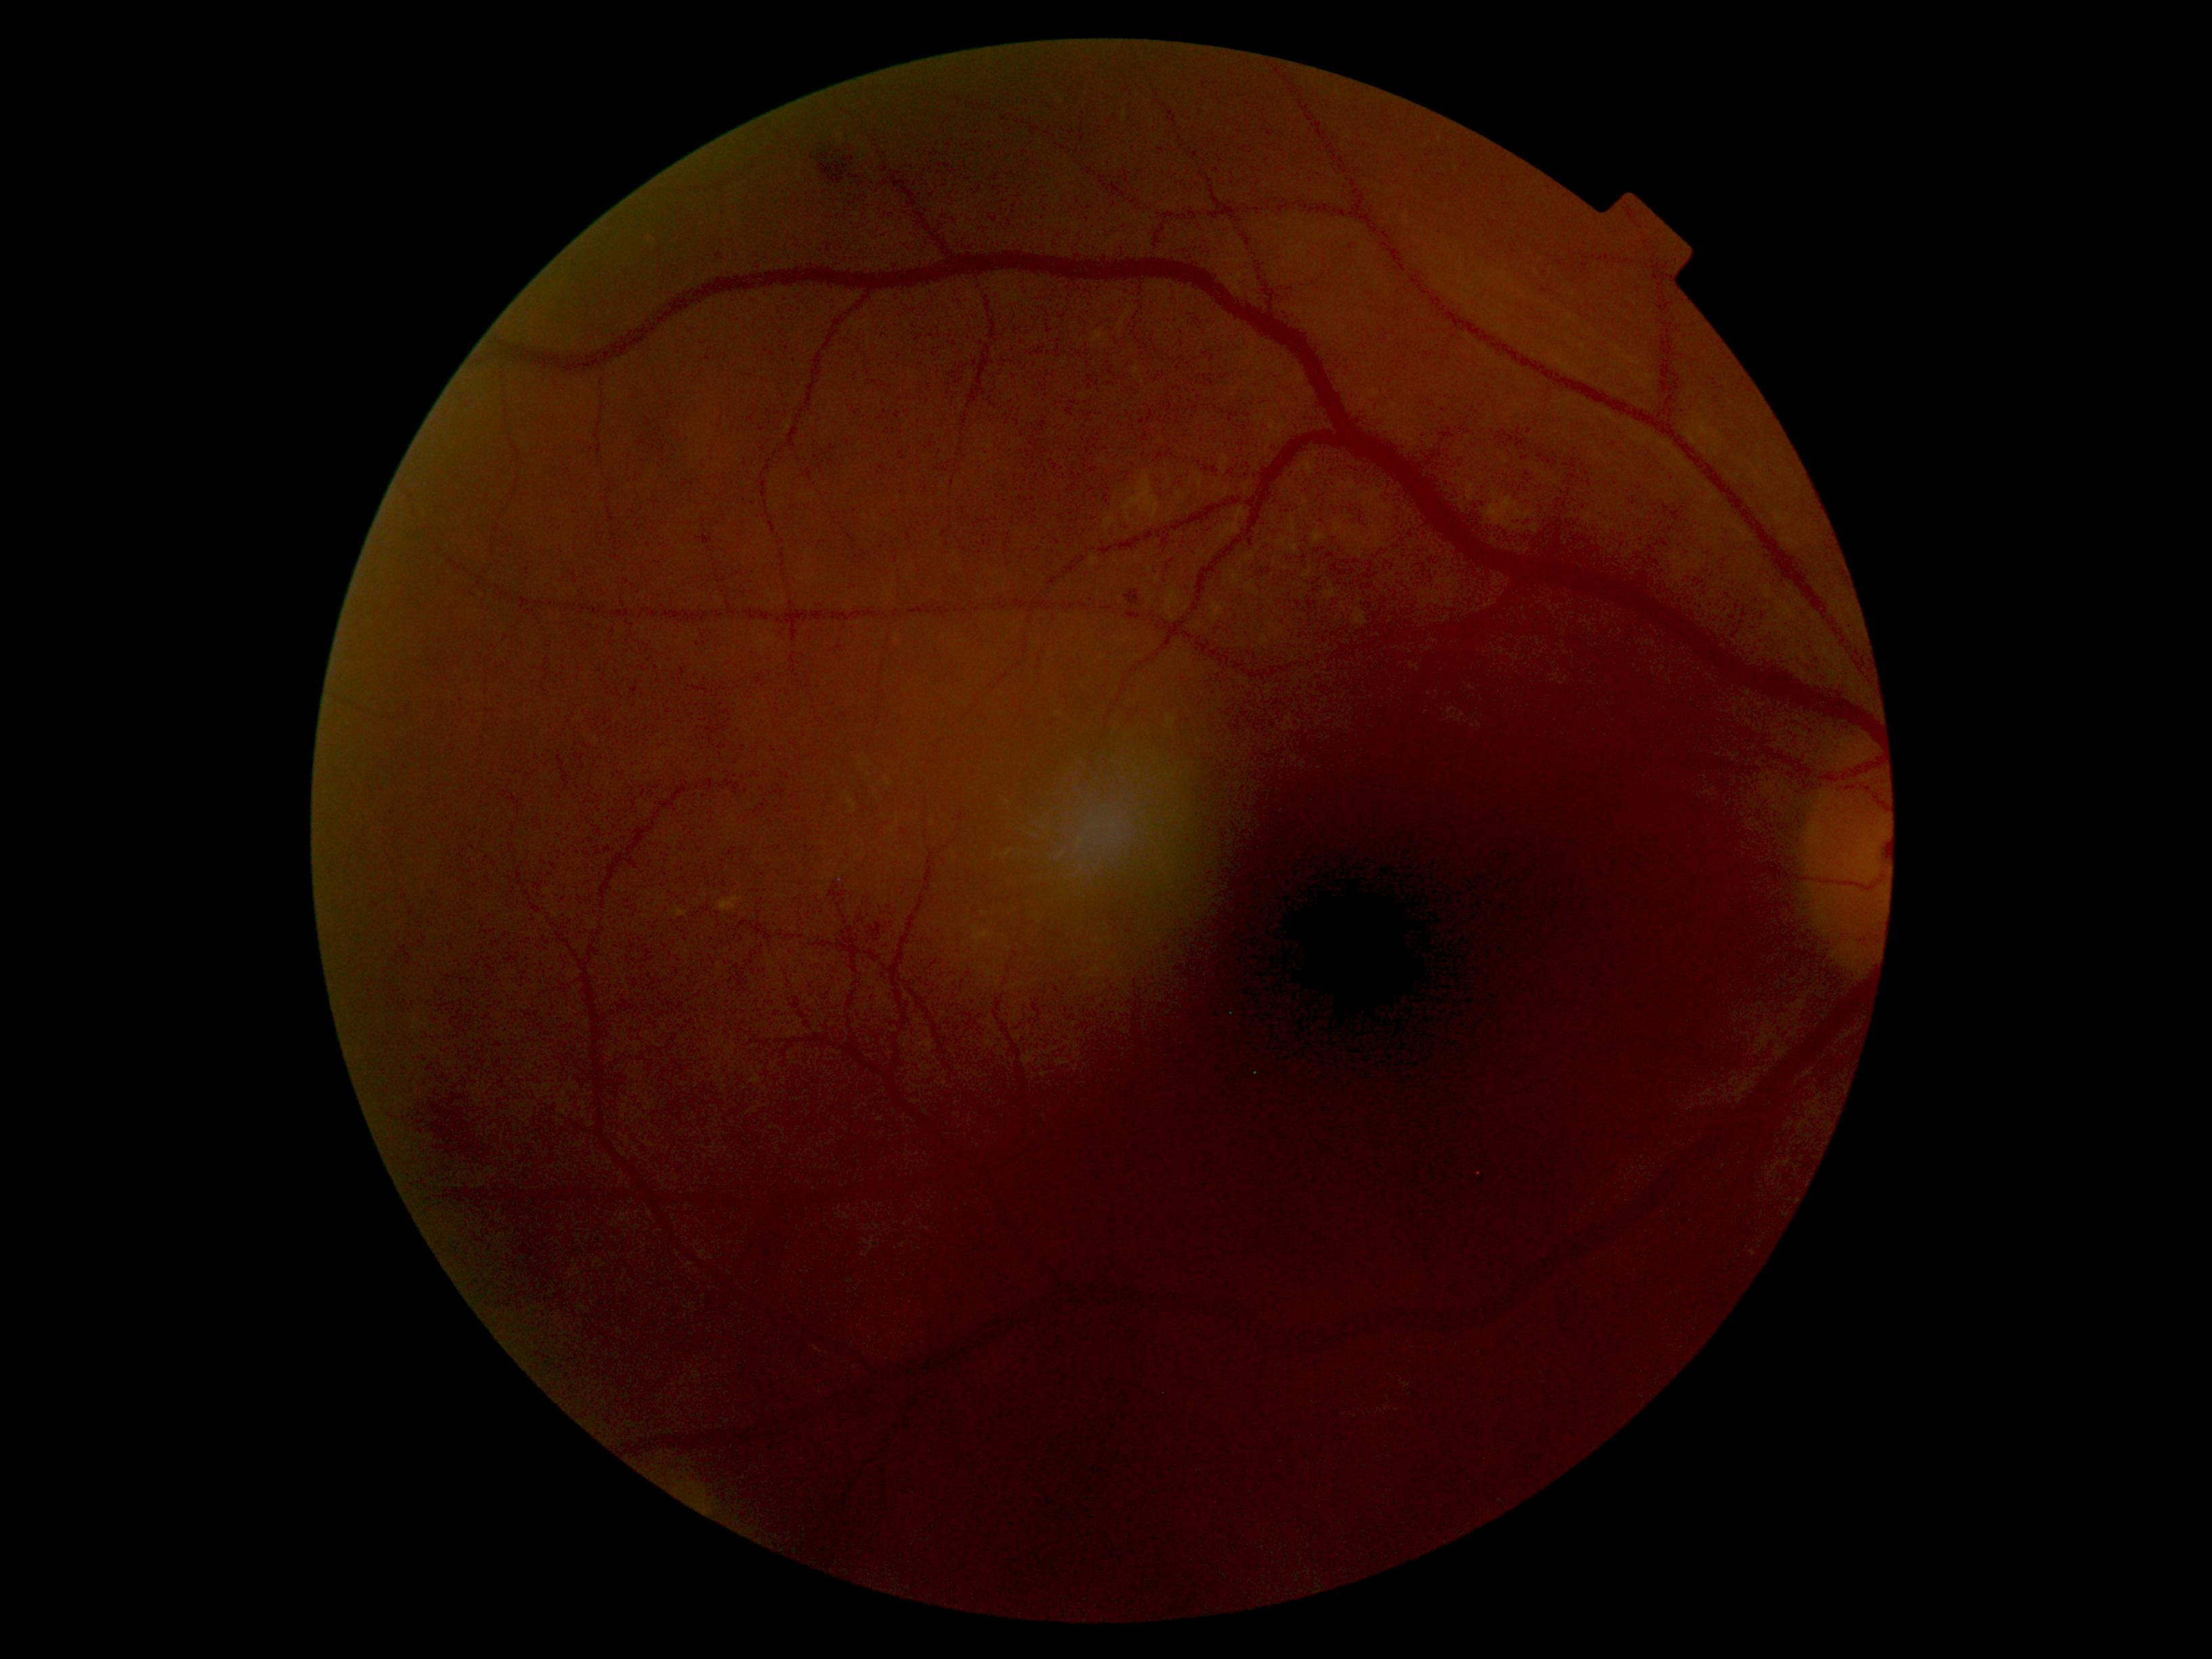
\includegraphics[height=\textwidth,width=\textwidth]{figures/chapter5/unconfident/35800_right.jpeg}
         \caption{Pred.: 2. Target: 2}
        \label{fig:unconfident3}
     \end{subfigure}
    \caption{Some images predicted with lower confidence (\( \leq 35\%\)) }
    \label{fig:unconfident}
\end{figure}

\subsection{Blending information from both eyes} \label{sec:blending} 
As we observed when exploring the dataset, there is high correlation between the DR grading of the left and right eye. We can use that correlation to \textit{blend} information coming from both eyes to create a prediction for each eye.

After trying different strategies for blending (as combining predictions from both eyes using a dedicated neural network) we opted for a feature-level approach, depicted in \Cref{fig:blended_model}.

In this approach, we use the CNN as a feature extractor for the left and right eye images. These features are concatenated and fed to a dense neural network, which generates a prediction for each eye. Compared to prediction-level blending, this strategy allows the classification of one eye to directly depend on features extracted on another eye.

We found that the strategy of using CNN as a feature extractor and adding detachable heads offered powerful and flexible solutions to different problems as blending or embedding extraction. Since heads are usually simple networks, they can be trained fast without significant computing cost.

In order to prevent overfitting, we used a heavily regularized network including \textit{dropout} after every layer and using LeakyReLU as an activation function. Blending both eyes' information provides a slight improvement over the simple classifier, increasing Kappa score by 0.018 points (from 0.80 to 0.818).

\begin{figure}[tb]
    \centering
    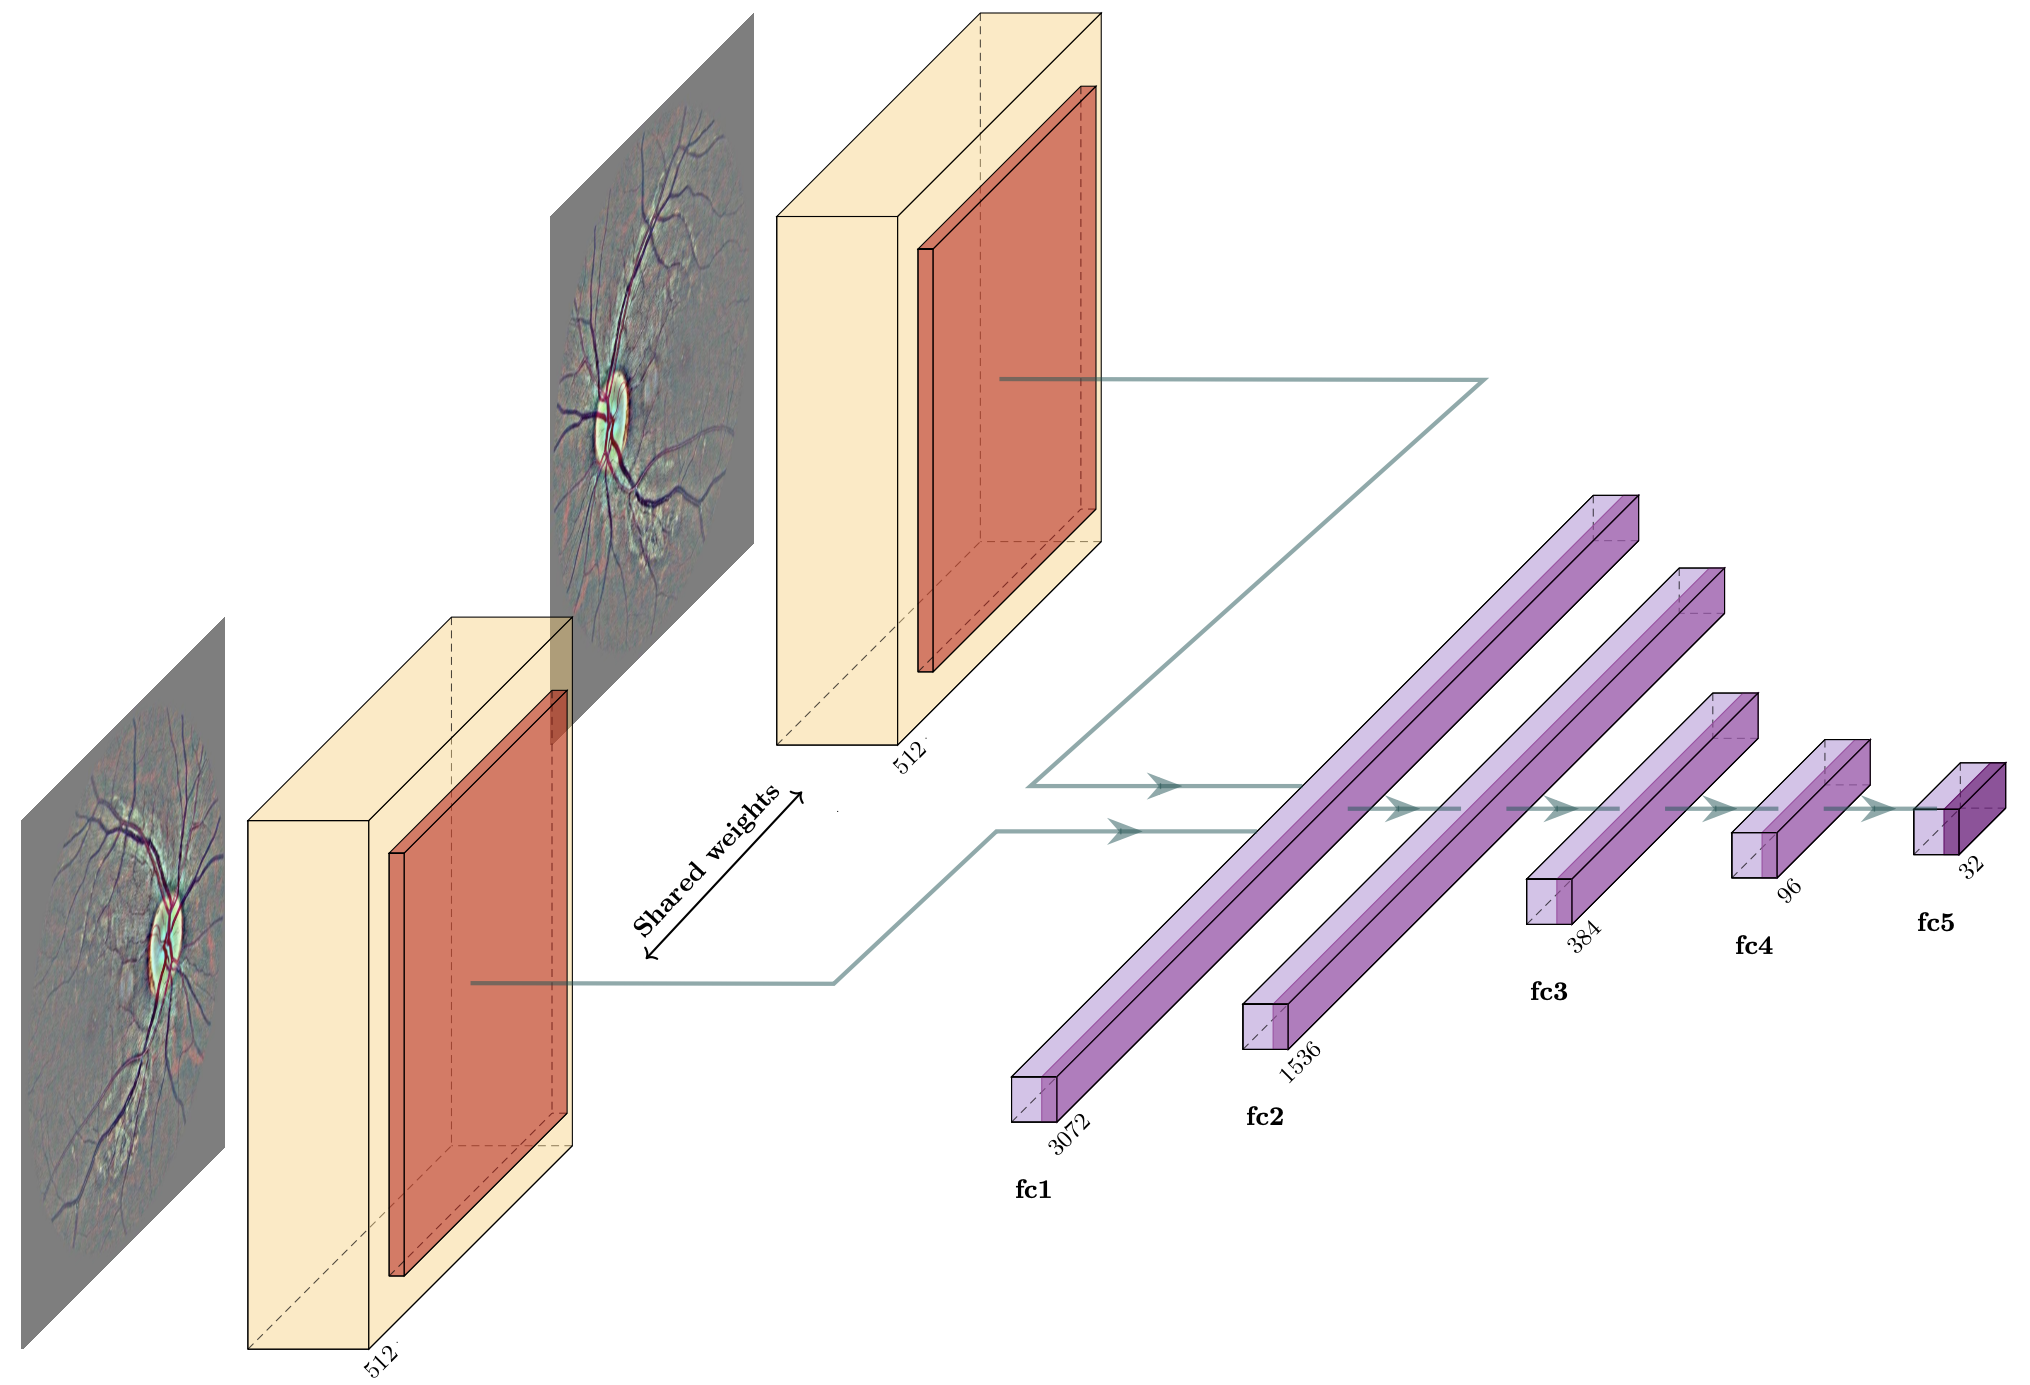
\includegraphics[scale=0.35]{figures/chapter5/models/blended_model.png}
    \caption{Architecture of the model for feature blending}
    \label{fig:blended_model}
\end{figure}

We also found that a slight improvement could be achieved by using a more sophisticated way to generate a class prediction from the model output. The result of processing an image is the (post-calibration) vector of logits \( y \), which represents the unnormalized probability for each class. Until this point, we generated the prediction as the class associated to the higher probability, which is especially convenient for validation, since this is a very fast process.

These probabilities can be normalized by applying \textit{softmax}. We then calculate the value \( \sum_{i = 0}^4 i y_i \) and obtain the prediction using a set of precomputed thresholds (0.57, 1.37, 2.30, 3.12), that we identified as providing the best \( \kappa \) score on the validation set using exhaustive search. Using this technique to generate predictions increased the \( \kappa \) score to 0.844, a very significant improvement.

To generate the final predictions we fed the model the test images by left and right pairs, each one rotated by a random angle and created five independent predictions. We obtained the final prediction by calculating \( \sum_{i = 0}^4 i \softmax(y_i^k) \) for each of the \( y^1, \dots, y^k \) vector of logits, averaging the results and using the previously found thresholds. We obtained a final kappa value of \( \kappa = 0.8491 \), which shows that generating multiple predictions is effective at improving performance.

\section{Model evaluation}
The obtained \( \kappa \) value would set us 2nd (out of 660 competitors) in the Kaggle competition for Diabetic Retinopathy Detection \cite{diabeticretinopathydetection}, which used the same setting. The first solution has a \( \kappa \) coefficient superior by less than \( 0.0005 \) and used an ensemble of three models, as almost all the dominant solutions did. While ensembles are a reliable way to improve performance, they are inconvenient since they increase training costs and, what is more important, multiply the time and resources needed for inference.

Our approach shows the viability of using pretrained smaller models to obtain excellent results in a computationally efficient way. The ROC curve, displayed in \Cref{fig:roc}, shows promising results with an area under the curve of 0.87 for referable cases (some sign of diabetic retinopathy) and 0.88 for severe cases (at least grade 3). 

\begin{figure}[tb]
     \centering
     \begin{subfigure}[b]{0.49\textwidth}
        \centering
        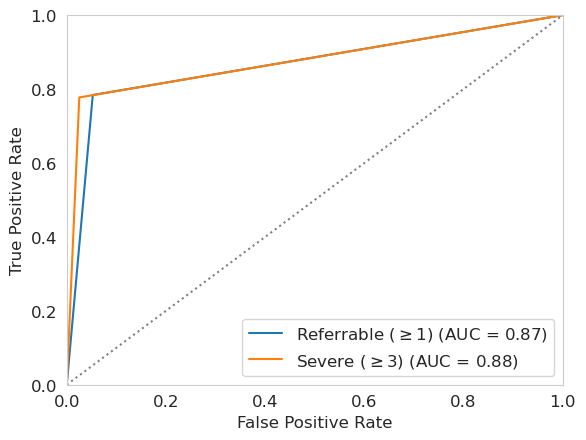
\includegraphics[width=\textwidth,height=.9\textwidth]{figures/chapter5/roc.png}
        \caption{ROC curve for referable cases (at least grade 1) and severe cases (at least grade 3)}
        \label{fig:roc}
     \end{subfigure}
     \hfill
     \begin{subfigure}[b]{0.49\textwidth}
        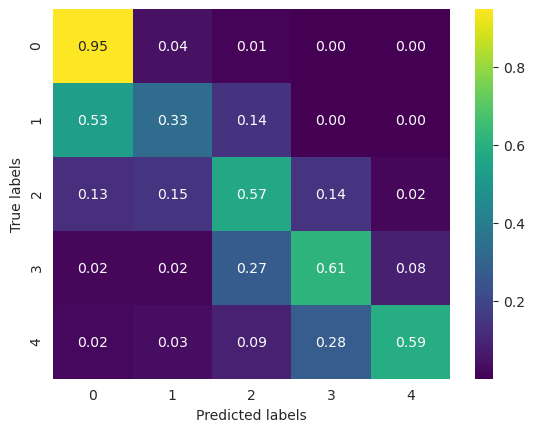
\includegraphics[width=\textwidth,height=.9\textwidth]{figures/chapter5/confusion.png}
        \caption{Confusion matrix for the obtained predictions}
        \label{fig:confusion}
     \end{subfigure}
     \hfill

    \centering
\end{figure}

The final level of accuracy is \( 83.31 \% \). The confusion matrix obtained is shown in \Cref{fig:confusion}. The performance is excellent over class 0 and reasonable solid over classes 2, 3 and 4. The difficulty to correctly detect the disease at grade \( 1 \) is in line with previous observations in the field about the complexity of correctly diagnosing intermediate classes. 

We must stress that the election of the thresholds for generating the final classification was intended to maximize the \( \kappa \) value, and they can and should be adjusted before applying the model to clinical practice, for example to reduce the rate of false negatives for grade 1 images.